\documentclass[10pt, preview]{standalone}
\usepackage{pgf,tikz}
\usepackage{amsmath}
\usepackage{amssymb}
\usetikzlibrary{shapes, arrows, arrows.meta, positioning}
\begin{document}
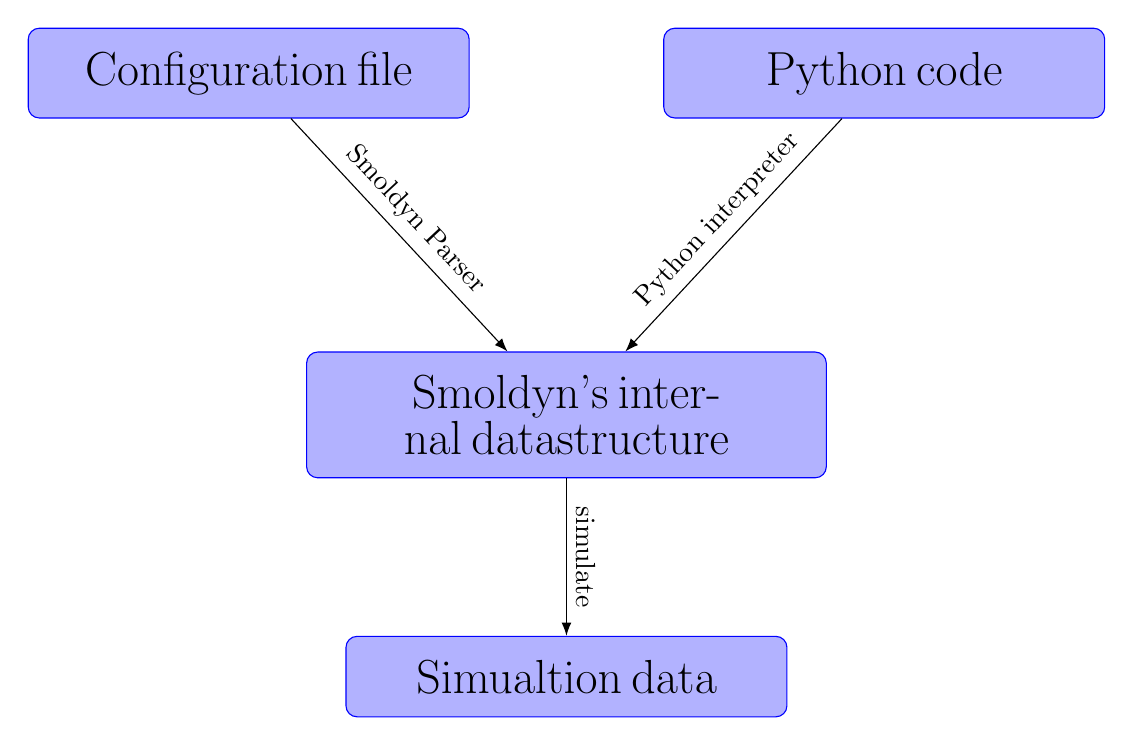
\begin{tikzpicture}[scale=1, transform shape]
    \tikzstyle{mystyle}=[text width=5cm, align=center, inner sep=3mm
    , rounded corners, draw=blue, fill=blue!30]
    \node[mystyle, text width=6cm] (struct) {\LARGE Smoldyn's internal datastructure};
    \node[mystyle, above left=5cm of struct, anchor=west] (config) {\LARGE Configuration file};
    \node[mystyle, above right=5cm of struct, anchor=east] (python) {\LARGE Python code};
    \node[mystyle, below=2cm of struct] (data) {\LARGE Simualtion data};

    % arrows
    \draw[-Latex] (config) to[] node[sloped, above]{Smoldyn Parser} (struct);
    \draw[-Latex] (python) to[] node[sloped, above]{Python interpreter} (struct);
    \draw[-Latex] (struct) to[] node[above, sloped] {simulate} (data);

\end{tikzpicture}
\end{document}          
